\documentclass[tikz,border=0]{standalone}
\usepackage[T1]{fontenc}
\usepackage{helvet}\renewcommand{\familydefault}{\sfdefault}
\usepackage{xcolor}
\definecolor{bg}{HTML}{171D2B}
\definecolor{ak}{HTML}{F7B538}
\definecolor{or}{HTML}{EF8354}
\definecolor{bl}{HTML}{7FB4E8}
\begin{document}
\pagecolor{bg}
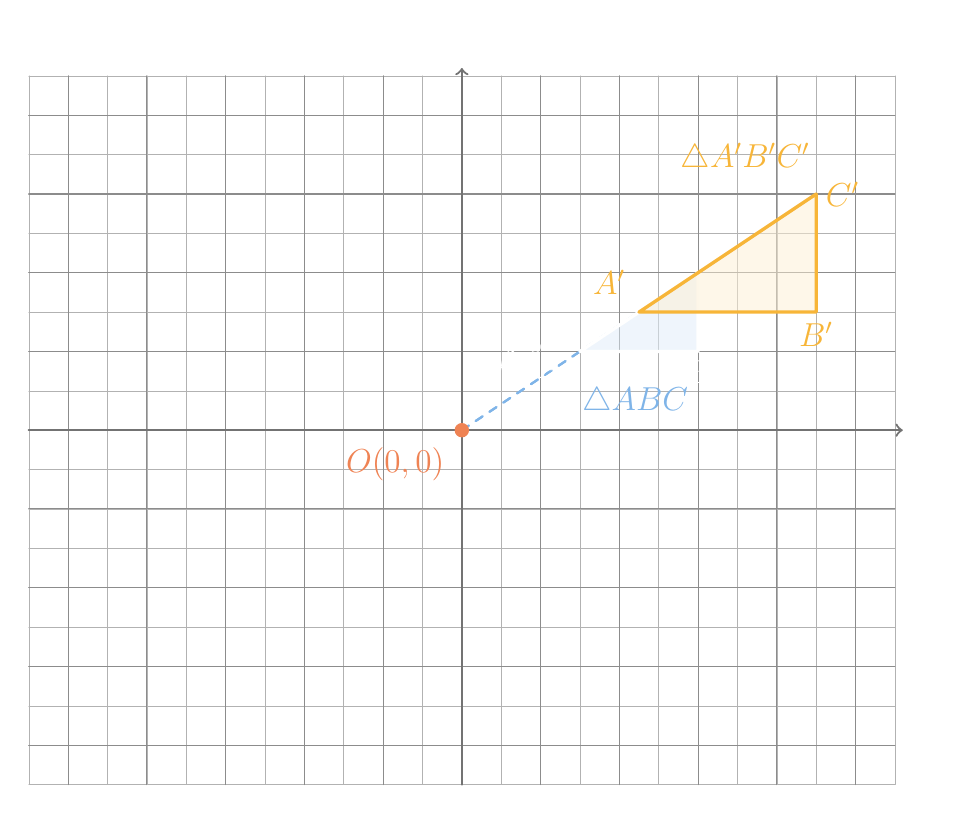
\begin{tikzpicture}[line cap=round,line join=round,x=1cm,y=1cm,
  every node/.style={text=white,font=\large}]

% grid halus
\draw[black!30,very thin] (-5.5,-4.5) grid[step=0.5] (5.5,4.5);
\draw[black!45,thin] (-5.5,-4.5) grid[step=1] (5.5,4.5);
\draw[black!55,thick,->] (-5.5,0) -- (5.6,0) node[right] {$x$};
\draw[black!55,thick,->] (0,-4.5) -- (0,4.6) node[above] {$y$};

% garis penyinar dari O
\draw[bl,thick,dashed] (0,0) -- (3,2);
\draw[bl,thick,dashed] (0,0) -- (4.5,3);

% segitiga asal
\draw[white,very thick,fill=bl!25,fill opacity=0.5] (1.5,1) -- (3,1) -- (3,2) -- cycle;
\node[bl] at (2.2,0.35) {$\triangle ABC$};

% segitiga bayangan
\draw[ak,very thick,fill=ak!22,fill opacity=0.5] (2.25,1.5) -- (4.5,1.5) -- (4.5,3) -- cycle;
\node[ak] at (3.6,3.45) {$\triangle A'B'C'$};

% titik pusat
\fill[or] (0,0) circle (2.6pt);
\node[or,anchor=north east] at (-0.1,-0.1) {$O(0,0)$};

% label titik asal
\node[white,anchor=east] at (1.4,0.8) {$A$};
\node[white,below] at (3,1) {$B$};
\node[white,anchor=south west] at (2.9,2.05) {$C$};
% label titik bayangan
\node[ak,anchor=south east] at (2.2,1.6) {$A'$};
\node[ak,below] at (4.5,1.5) {$B'$};
\node[ak,right] at (4.5,3) {$C'$};

% keterangan faktor skala pada garis penyinar
\node[white,font=\normalsize,rotate=33.7,anchor=south] at (0.85,0.68) {$\times 1{,}5$};

\end{tikzpicture}
\end{document}
